%
\documentclass[Proceedings]{ascelike}
%
% Feb. 14, 2013
%
% Some useful packages...
%
\usepackage{graphicx}
%\usepackage{subfigure}
%\usepackage{amsmath}
%\usepackage{amsfonts}
%\usepackage{amssymb}
%\usepackage{amsbsy}
%\usepackage{times}
%
%
% Place hyperlinks within the pdf file (works only with pdflatex, not latex)
% \usepackage[colorlinks=true,citecolor=red,linkcolor=black]{hyperref}
%
%
% NOTE: Don't include the \NameTag{<your name>} if you have selected 
%       the NoPageNumbers option: this leads to an inconsistency and
%       a warning, and the NameTag is ignored.
%\NameTag{Kuhn, Feb. 14, 2013}
%
%
\begin{document}
%
% You will need to make the title all-caps
\title{Determinaci\'on de la orbita de una estrella binaria espectrosc\'opica.}
%
\author{
Nicolas Garavito-Camargo%
%
% ---- The first of two styles for addresses: using footnotes and \thanks ----
\thanks{
Dept.\ de F\'isica.,
Universidad de los Andes, 
Calle 1...\ Bogot\'a, Colombia. E-mail: jn.garavito57@uniandes.edu.co}
\ Benjamin Oostra\footnotemark[1]
%
% Adding a second author with the same affiliation (still using \thanks):
%  \\
 %Colleague,\footnotemark[1] Member, ASCE%
%
% Adding another author with a different affiliation.  I have found that 
% the \and command doesn't quite work, so just use "and", as in the following 
% \\
% and
% Younyee Kuhn%
% \thanks{Flourishing wife of same.},%
% \ Not a Member, ASCE
%
% ---- The second of two styles for addresses: below names, no footnotes ----
%
% For this style, don't use \thanks.  Instead, use superscripts and carriage
% returns ("\\").  It's not pretty, but neither is the new ASCE proceedings
% style.  Something like the following:
%
% Matthew R. Kuhn$^1$, Member, ASCE\\[1ex]%
%
% $^1$\parbox[t]{5.75in}{Dept.\ of Civil Engrg.,
% Donald P.\ Shiley School of Engrg., Univ.\ of Portland, 
% 5000 N.\ Willamette Blvd., Portland, OR  97203. kuhn@up.edu.}
}
%
\maketitle
%
\begin{abstract}

\end{abstract}


%
% Some keywords, using a new command: \KeyWords{}
%
\KeyWords{..}
%
\section{Introducci\'on}

En astronomia a diferencia de la f\'isica no hay experimentos que realizar,
solo se tiene un universo al cual observar. Se puede hacer simulaciones sobre 
fen\'omenos astrofisicos que al final den cuenta de las observaciones.

Estas observaciones son de la radiaci\'on que nos llega del universo y pueden 
realizarse en diferentes longitudes de onda del espectro electromagnetico.  

\subsection{Espectrografia}

La espectrografia es una tecninca en la cual la luz se descompone en las diferentes
longitudes de onda y a partir de las intensidad de las diferentes lineas de emision/absorcion
se encuentras cantidades fisicas importantes de los objetos celestes observados.

a partir de mediciones del espectros tomados en el observatorio de la universidad 
de los andes se pretende reconstruir la orbita de una estrella binaria en este caso 
se selecciono Epsilon de la corona australis. La importancia de medir orbtias en astronomia
radica en de estas poder reconstruir los potenciales gravitacionales que goviernan 
dichos objetos.

\subsection{Clasificacion espectral de las estrellas}

Las estrellas se clasifican segun

\section{Seleci\'on de la binaria a observar}

Para la seleci\'on de la estrella binaria a observar se tuvieron en cuenta 
diferentes caracteristicas tales como:

\begin{itemize}
\item Visibilidad en nuestra posicion (poner coordenandas)
\item Magnitud aparante
\item Longitud del periodo
\item Clase espctral
\end{itemize}


\section{Epsilon Coronae Australis}

Epsilon Coronae Australis ($\mathrm{\epsilon}$ CRA) ubicada en la 
constelcion de la Coronae Asutralis, es una binaria eclipsante \\

\begin{tabular}{c c}
\hline
Principales Caracteristicas\\
\hline
\hline
Asencion Recta & 18h58m43.5s \\
Declinacion & $-37^{0}$06'18'' \\
Periodo Orbital & 0.59 d\'ias \\
Magnitud & 4.83 \\
Clase espectral & F2 \\
Distancia entre estrellas & 2.9 Millones de Km\\ 
\hline
\hline
\end{tabular}

\begin{center}

\begin{figure}
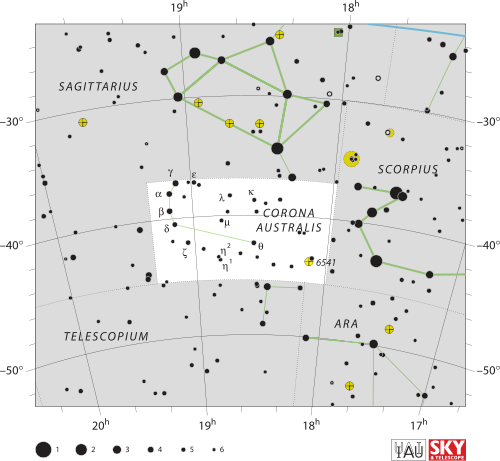
\includegraphics[scale=0.4]{CRA.png}
\caption{Corona Australis, http://www.iau.org/static/public/constellations/gif/CRA.gif \label{la}}
\end{figure}
\end{center}

\section{Observaciones}

Todas las observaciones se han llevado acabo en el observatorio astronomico de la 
Universidad de los Andes. A continuaci\'on se describen la instrumentacion utlizada
as\'i como los protocolos de observaci\'on utilizados.

\subsection{Instrumentaci\'on}

\subsubsection{Telescopio}

Se utilizo un telescopio marca Meade LX200 Schimdt-Cassegrain de $40 cm$ de apertura y una
distancia focal de $4m$

\begin{figure}
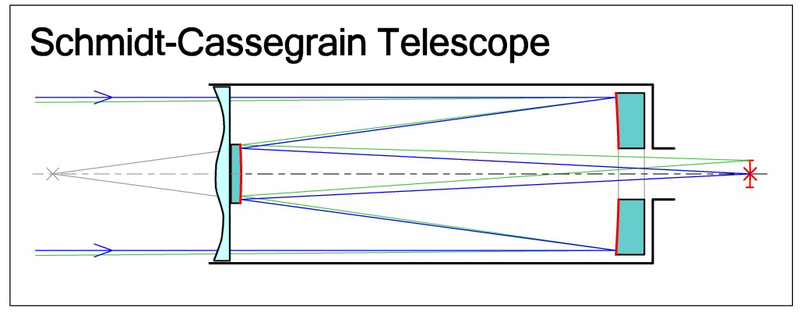
\includegraphics[scale=0.4]{SCT2.jpg}
\caption{Camino de luz en un telescopio Schmidt-Cassegrain, http://en.wikipedia.org/wiki/File:Schmidt-Cassegrain-Telescope.png \label{la}}
\end{figure}

\subsubsection{Espectrografo}

\subsubsection{Software}

\subsection{Protocolo de Observacion}

Todas las observaciones se han llevado acabo en un intervalo de tiempo aproximadamente 
desde las 5pm hasta las 9 pm.

\section{Resultados preliminares}

\section{References}

http://ned.ipac.caltech.edu

\end{document}
